\documentclass[thesis.tex]{subfiles}
\usepackage{multirow}
\usepackage{amsmath}
\usepackage{graphicx}

 
\begin{document}
\chapter{Experimental Apparatus}

\section{The Large Hadron Collider}
The Large Hadron Collider (LHC), located at CERN on the France-Switzerland border, is currently the world's largest particle accelerator and collider. 
It is installed in a 27 km long near-circular tunnel that was constructed in the 1980s to host the Large Electron-Positron (LEP) machine. 
The LHC uses twin-bore magnets to allow two proton beams to travel in opposite directions. 
The main superconducting magnets of the LHC operate at a temperature below 2K, which is maintained by a superfluid helium cryogenic system, and generates a peak dipole field of 8.33 T. 
The LHC is designed to provides a peak luminosity of $L = 10^{34}cm^{2}s^{-1}$ and a maximum center of mass energy of $\sqrt{s} = $14 TeV for proton-proton collisions.  \\

The protons injected to the LHC are boosted by a chain of accelerators, each of which increases the energy of the protons to a certain scale and the beams can also be delivered to other experiments at low energy. 
The configuration of the CERN accelerator complex is shown in Fig. 2. 
At the first stage, the protons extracted from a bottle of hydrogen gas are fed into the LINAC 2, a linear accelerator, and are boosted to the energy of 50 MeV.  
The beams are then injected to the Proton Synchrotron Booster, followed by the Proton Synchrotron (PS), which brings the protons to 25 GeV. 
The Super Proton Synchrotron (SPS) then accelerates the proton beams to 450 GeV and injects them into the LHC. 
The LHC is the last element in the accelerator complex, where protons are stored and accelerated to the designed energy. \\

The two high-energy proton beams circulate in the LHC at close to the speed of light and collide with each other at four interaction points (IP), corresponding to the location of the four detector: CMS, ATLAS, ALICE and LHCb. 
The CMS and ATLAS are general-purpose detectors, which investigate a wide range of physics from the precise measurements of the SM to searches for new physics. 
The ALICE is a heavy-ion detector, focusing on the study of strong interactions. 
The LHCb experiment specializes in b quark physics, and it is a single arm detector which mainly collect forward particles. 
In addition, there are three smaller experiments on the LHC: TOTEM (Total, elastic and diffractive cross-section measurement), LHCf ((Large Hadron Collider forward) and MoEdal (Monopole and Exotics Detector). 
This thesis will focus on the results of the CMS experiments. 

\section{The CMS Detector}

The Compact Muon Solenoid (CMS) experiment is a hermetic, general-purpose detector located at the collision point 5 of the LHC.  It is 21.6 m long, 15 m high , 15 m in diameter, and weights about 12,500 tons. The physics goal is to investigate a wide range of phenomena including the study of the Higgs mechanism and searches for unknown particles beyond the SM. The cross-section of the interesting physics process is typically 5-10 order of magnitude smaller than the total cross-section, making it crucial to measure the momentum and time of the particles with high resolution. To meet the physics goals, the detector is designed to fulfill the following requirements:   
\begin{itemize}
\item good muon identification and high momentum resolution;
\item good electromagnetic energy resolution;
\item efficient tracking and accurate momentum measurements for charged particles;
\item good missing transverse momentum resolution, requiring hadron calorimeters with a large hermetic geometric coverage. 
\end{itemize}

To satisfy these requirements, a 13 m long, 6 m inner diameter superconducting solenoid is built to generate a magnetic field of 4 T, providing large bending power to precisely measure the momentum of charged particles. The coil is cooled by liquid helium to operate at an temperature of 4.5 K. The flux is returned through a steel yoke consisting of five barrel wheels and four end-cap disks at each end. \\

Figure 3 shows an overview of the layout of the CMS detector. Close to the interaction point is a high granular three-layer silicon pixel detector which improves the track and vertex reconstruction, followed by a silicon strip tracker. Surrounding it is a lead-tungstate crystal electromagnetic calorimeter (ECAL) and a brass/scintillator sampling hadron calorimeter (HCAL). The tracker and calorimeter are compact enough to fit into the bore of the magnet coil. Outside the solenoid are the muon stations, embedded in the return yoke. \\

The CMS uses a coordinate system with the origin centered at the interaction point. The positive y-axis is chosen to be the vertically upward direction, and the x-axis points toward the center of the LHC. Therefore the z-axis is pointing along the anti-clockwise beam direction. Cylindrical coordinates (r,$\phi$) are often used to described the transverse plane, with $\phi$ being the azimuthal angle measured from the x-axis and r being the radial coordinate in the plane. The momentum and energy in the transverse plane, denoted as $p_T$ and $E_T$, are usually used as kinematic variables for physics objects, because the transverse components are invariant under Lorentz boosts in the z direction. The polar angle $\theta$ is measured from the z-axis, and the pseudo-rapidity is defined as: \\
       $\eta = -ln tan(\theta/2)$.
       
\subsection{The Inner Tracking System}
The tracking system is designed to provide a precise and efficient reconstruction of the trajectories of charged particles. 
At the same time, accurate measurements of secondary vertices and impact parameters are necessary for the estimation of the positions of primary vertices as well as the identification of heavy flavors. 
At the designed luminosity of the LHC, about 1000 particles are expected to hit the tracker at each bunch crossing. 
To keep the occupancy at around 1\% in such challenging operation conditions, pixelated detectors and micro-strip detectors are used at the small radii and large radii regions respectively. 
The sensors are solely made of radiation tolerant silicons. With a sensitive area of about 200 $m^2$, the CMS tracker is so far the largest silicon tracker.  \\

The tracker has a cylindrical volume of 5.8 m in length and 2.5 m in diameter, embedded in the homogeneous magnetic field of 3.8 T. 
A schematic view of the CMS tracker is shown in Fig. 4. 
In the barrel region, the pixel detector consists of three cylindrical layers at radii between 4.4 cm and 10.2 cm and the strip tracker consists of ten layers extending to 110cm in radius. 
Both subdetectors are complemented by disks on each side, extending to 290 cm in z and covering a pseudorapidity range up to $|\eta| <$ 2.5.  \\

The pixel detector consists of three barrel layers located at radii of 4.4, 7.3 and 10.2 cm, closed by two disks on each side at z = $\pm$ 34.5 and $\pm$ 46.5 cm. 
It contains a total number of about 66 million silicon pixels with cell size of 100 $\times$150 $\mu m^2$. 
It provides good track resolution in both the r-$\phi$ and z directions, allowing a three-dimensional (3-D) vertex reconstruction. 
It is essential for the identification of heavy flavors and forming seeds for the track finding. \\

Surrounded the pixel system is the strip tracker. 
It is composed of four subsystems. 
The Tracker Inner Barrel (TIB) and Disk (TID) extend to a radius of 55cm, and are composed of four barrel layers and three endcap disks on each side. 
The sensors used by the TIB/TID are 320 $\mu m$ thick silicon micro-strips. 
The strips in the barrel are parallel to the beam pipe and have a pitch of 80 $\mu m$ on layer 1,2 and 120 $\mu m$ on layer 3,4, providing a position resolution of 23-35 $\mu m$. 
The disks use wedge-shaped sensors, with a pitch varies between 100 $\mu m$ and 141 $\mu m$. 
The innermost two layers of the TIB and the first two rings of the TID also carry a second module, mounted back-to-back with a stereo angle of 100 mrad, in order to measure the z (r) coordinate in the barrel (disks). \\

The Tracker Outer Barrel (TOB) covers the radius from 55 cm to 116cm and consists of six barrel layers, with the innermost two layers having double-modules. 
The sensor are made of 500 $\mu m$ thick micro-strips, with pitches vary from 183 $\mu m$ to 122 $\mu m$. 
The TOB covers z $<$ 118 cm. The rest of the tracker volume is occupied by the Tracker Endcaps (TEC), composed of 9 disks on each side. 
300 $\mu m$ silicons are used on the inner fours rings, and 500 $\mu m$ thick strips are used in the outer rings. \\

%Figure 5 shows the tracker material budget as a function of \eta, as estimated from simulation. The tracker modules, together with electronics, cooling and support structures, contribute a large amount of materials in the tracker volume and cause particles to interact before reaching the outermost layer of the tracker. 

Figure 5 shows the resolution of the pixel and strip detectors during the Run-II operation. A 8~10 $\mu m$ $r-\phi$ and 20-25$\mu m$ resolution was achieved in the pixel barrel. 

\subsection{Electromagnetic Calorimeter}
The CMS electromagnetic calorimeter (ECAL) is a hermetic, homogeneous detector consisting of 61,200 PbWO$_4$ crystals in the barrel (EB), and 7324 crystals in each of the two endcap sections (EE). 
The PbWO$_4$ crystals have a density of 8.28 g/cm$^3$, radiation length of 0.89cm and Moli`ere radius of 2.2 cm. 
These characteristics make them the appropriate material for a compact calorimeter. 
The scintillation light emitted by the crystals are blue-green color, with a maximum wave length at 420-430 nm. 
Therefore blue laser can be used to monitor the transparency and response of the crystals. 

The scintillation light is collected by avalanche photodiodes (APDs) in the barrel section and vacuum phototriodes (VPT) in the endcaps. 
Each barrel crystal has one pair of APDs glued to its back face, and each endcap crystal has only one APT mounted. 
The photodetectors are depleted by a custom high voltage (HV) power supply which can precisely control the bias voltage and allow the gain of the photodetectors to be stable. 

A schematic drawing of the layout of the ECAL is shown in Figure 6. 
The EB uses 230 mm long crystals, corresponding to a radiation length of 25.8 $X_0$, whilst the length of the crystals in the EE is 220 mm (24.7 $X_0$). 
The crystals in the EB are grouped into 36 supermodules (SM), 18 on each side of the interaction point, and provide a granularity of 360-fold in $\phi$ and (2$\times$85)-fold in $\eta$, covering the pesudorapidity range up to $|\eta| <$ 1.479. 
The EE is composed of two Dees, each consists of 3662 crystals, and extends the coverage to $|eta| = $3.0. 
In addition, a preshower (ES) detector made of lead absorbers and silicon strip sensors is placed in front of EE to improve the identification of closely spaced photons from $\pi^0$ decays. 

The signals from the photodetectors are shaped and amplified by the Multi Gain Pre-Amplifier (MGPA) with gains of 1, 6 and 12. 
If the signal is saturated, the read-out will switch to a lower gain. 
Each of the output signal of the MGPA is digitized by a 12 bit analog-to-digital converter (ADC) running at 40MHz and a set of 10 consecutive samples is recorded for amplitude reconstruction.
The signals from a trigger tower ( $5\times5$ crystals ) in the EB or a super-crystal in the EE are read out together by the on-detector electronics and are stored in pipelines during the Level-1 trigger latency. 
Once a Level-1 trigger is received, the data will be sent out to the off-detector electronics. 

Radiation can cause a degradation in the crystal transparency due to the formation of color centers. 
The response of the VPT also varies under irradiation. 
In absence of irradiation the transparency loss can partially recover through spontaneous annealing. 
These response changes are measured and corrected using a laser based light monitoring system during the LHC operation. 
Blue and green laser light pulses are injected via optical fibers to the crystals and off-detector silicon PN photodiodes. 
The relative responses are then normalized to the measurements at the start of the run to derive correction coefficients. 
Figure \ref{fig:lasermonitor} shows the evolution of the ECAL response for the Run I and Run II 2016 data taking periods. 

\begin{figure*}[hbtp]
	\centering
	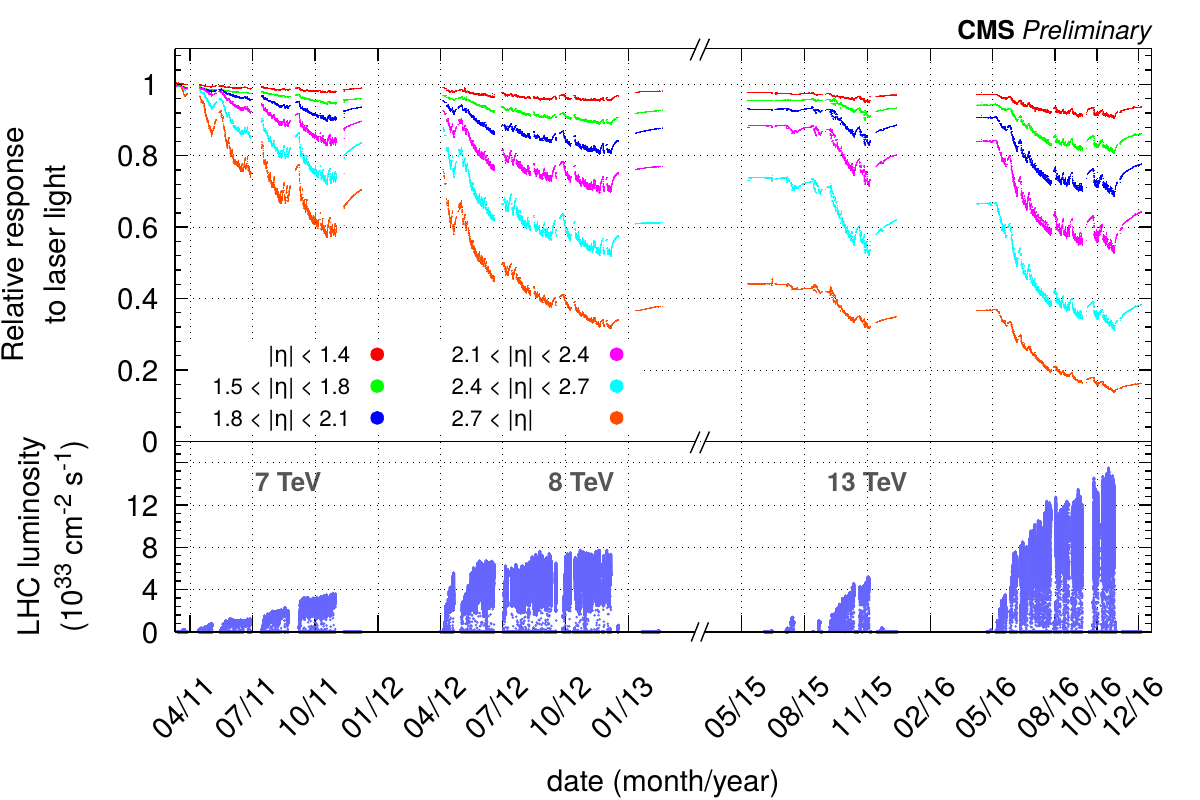
\includegraphics[width=0.8\textwidth]{plot/lasermonitor.png}
\end{figure*}

The ECAL has been operating stably throughout the 2015 and 2016 LHC Run II operation.
The analysis using 2.5fb collision data collected in 2015 shows that a relative energy resolution
between 1.4\% and 3\% for electrons is achieved in the EB, and 3\% to 4\% for EE. The resolution for
low and high bremsstrahlung electrons are shown in Figure \ref{fig:ecalreso}.

\begin{figure*}[hbtp]
	\centering
	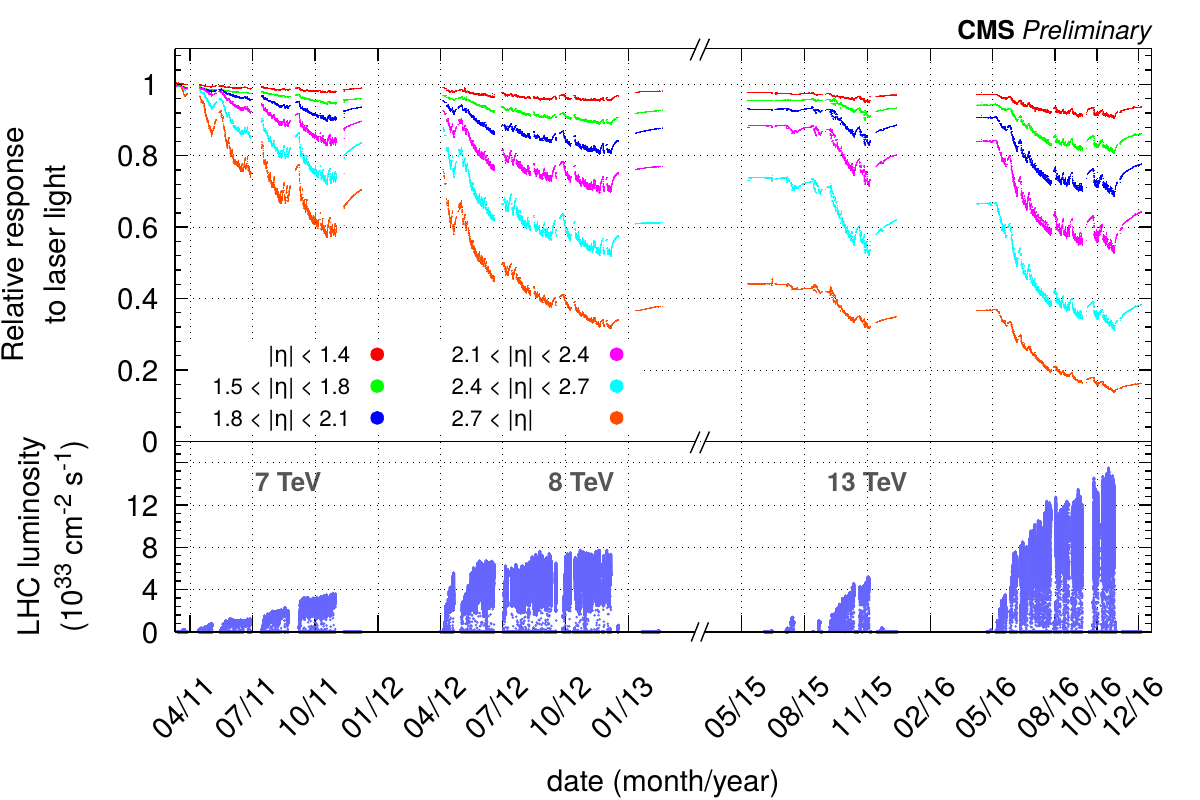
\includegraphics[width=0.8\textwidth]{plot/lasermonitor.png}
\end{figure*}

\section{The CMS Trigger System}

\section{The CMS Data Acquisition System}

\section{The Data Quality Monitoring and Certification System}


\end{document}


